\begin{frame}[allowframebreaks]
	\par The liquid state machine (LSM) has emerged as a computational model that is more suitable than Turing machines for describing neural networks. It is used to process continuous streams of data, typically in the form of spike trains, and it maps streams of inputs into streams of outputs. These outputs may depend on the previous states created by the streaming data \cite{doi:10.1142/9781848162778_0008}.
	
	\par LSM is model for adaptive computing systems. Considering that the training stage is the most expensive and sensible one, these kind of networks are trained only at the readouts. These readouts, usually, consists of only a single neuron which is called \textit{"projection neuron"} that extracts information from a micro-circuit somewhere in the LSM. These structures can be used as inputs to another area of the neural network and can be modeled as a perceptron, linear gate, sigmoidal gate, spike neuron and others \cite{doi:10.1142/9781848162778_0008}. The networks structure consists of several neurons randomly and recurrently connected forming the \textit{"liquid part"} which is interpreted by the readouts. The word \textit{"liquid"} can sometimes be take literally like in this work \cite{10.1007/978-3-540-39432-7_63} where a bucket of water has been taken the role of the liquid part of the network as can be seen in Figure \ref{fig:leterallyaliquidnetwork}.
	
	\begin{figure}
		\centering
		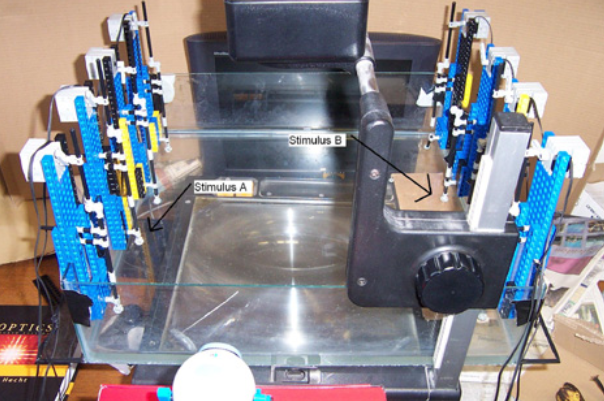
\includegraphics[width=0.7\linewidth]{images/leterallyALiquidNetwork}
		\caption[A liquid network]{A liquid network. Source: \cite{10.1007/978-3-540-39432-7_63}}
		\label{fig:leterallyaliquidnetwork}
	\end{figure}
	
	
	
	
	
	\par LSM can be adapted to multiple computation as the projection neurons can extract as many different characteristics one desires as can be seen in Figure \ref{fig:projectionneurons}.
	
	\begin{figure}
		\centering
		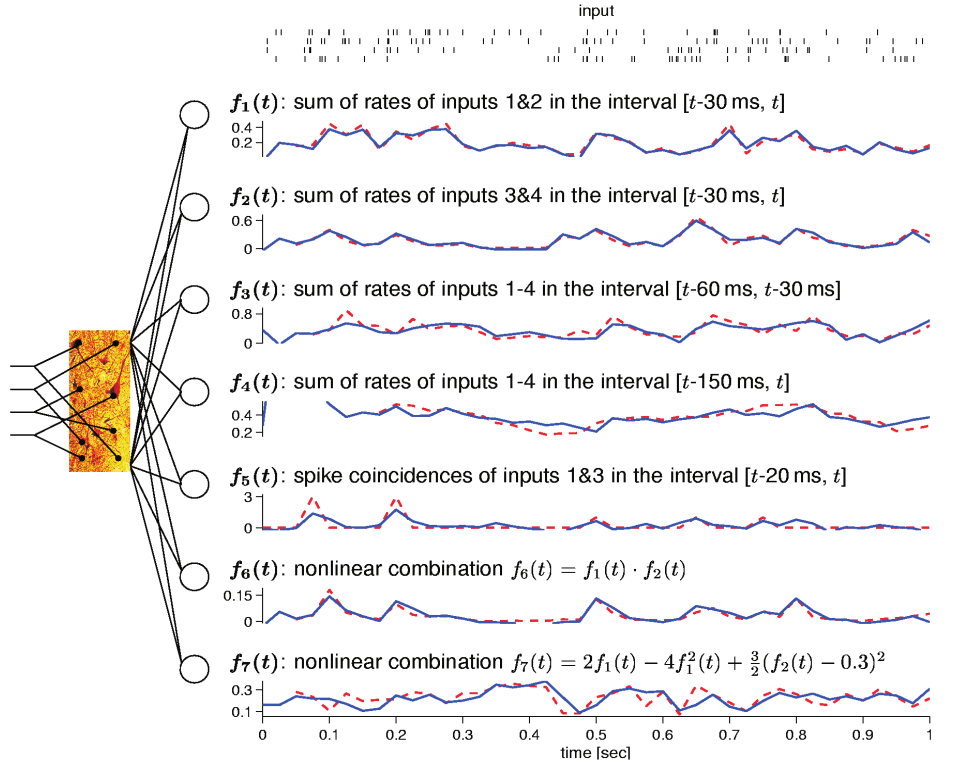
\includegraphics[width=0.7\linewidth]{images/projectionNeurons}
		\caption{}
		\label{fig:projectionneurons}
	\end{figure}

	
	
	
\end{frame}